Swapping Assignments between Multiple Views (SWAV) \cite{caron2020unsupervised} unlike all the other methods we've seen, it does not use contrastive learning but it is an online clustering based method. In clustering based method the idea is to use a clustering algorithm to cluster the embedding of a batch of images, and use those embedding as pseudo-label for a predictive task in which a model given the embedding of the images is trained to predict the cluster of each image. This method was proposed in Deep Cluster \cite{caron2018deep}.
\begin{figure}[H]
	\centering
	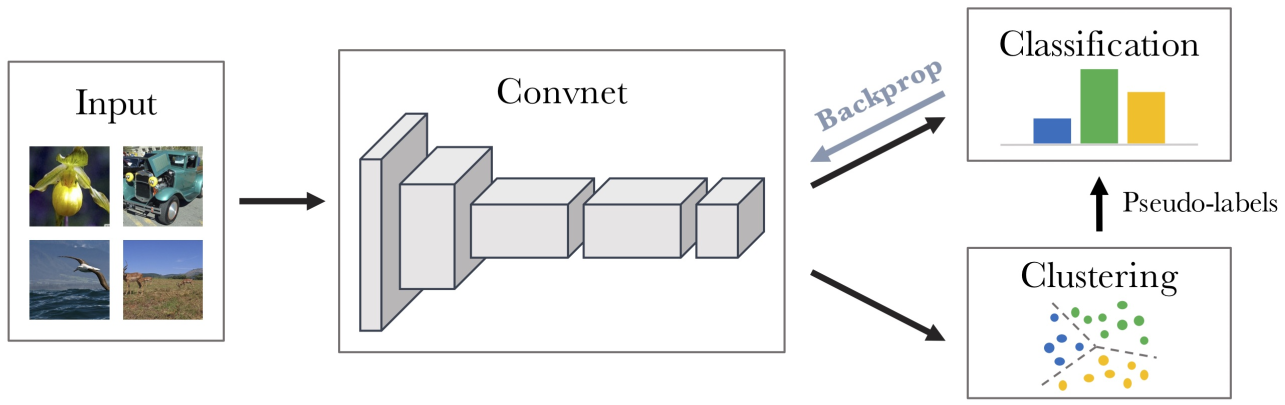
\includegraphics[width=10cm]{./images/deep_cluster.png}
	\caption{General framework of clustering based methods}
\end{figure}

With SWAV the authors combine the main framework of contrastive learning, which is comparing different views of the images produced with augmentation, with a clustering based pretext task. SWAV works as follows: each image $x_n$ is transformed into an augmented view $x_{nt}$ by applying a transformation $t \sim \mathcal{T}$, where $\mathcal{T}$ is a set of augmentations. Then we map the augmented view to a vector representation with a non-linear mapping $f_\theta$ to $x_{nt}$ and we then project this feature in a unit sphere $z_{nt} = f_\theta(x_{nt})/\lVert f_\theta(x_{nt}) \rVert_2$. From this representation we compute the code $q_{nt}$ by mapping $z_{nt}$ to a set of $K$ trainable prototypes vectors $\{c_1, \dots, c_k\}$. We use $C$ to denote the matrix whose columns are the $c_1, \dots, c_k$ vectors. If we do the same thing with another augmentation $s \sim \mathcal{T}$, obtaining the image feature $z_{ns}$ and its corresponding code $q_{ns}$ then we can set a swapped prediction problem using the following loss:
\[ L(z_{nt}, z_{ns}) = \ell(z_{nt}, q_{ns}) + \ell(z_{ns}, q_{nt}) \]
where the function $\ell(z, q)$ measures the fit between features $z$ and the code $q$. The idea is that instead of comparing directly the features of $z_t$ and $z_s$, we do it using the intermediate codes $q_t$ and $q_s$. If these two features capture the same information, it should be possible to predict the code of the feature $z_q$ using the feature $z_t$ and vice versa. The loss $\ell(z_t, q_s)$ is the cross entropy loss between the code and the probability obtained by taking a soft-max of the dot product of $x_i$ and all the prototypes in $C$:
\[\ell(z_t, q_s) = -\sum_k q_s^{(k)}\log p_t^{(k)}, \qquad p_t^{(k)} = \frac{\exp(z_t^Tc_k/\tau)}{\sum_{k^\prime}\exp(z_t^Tc_k^\prime/\tau)}\]
by applying some mathematical manipulations to these formula we can obtain our objective: 
\[\frac{1}{N}\sum_{n=1}^N \sum_{s, t \sim \mathcal{T}}L(z_{nt}, z_{ns}) = -\frac{1}{N}\sum_{n=1}^N \sum_{s, t \sim \mathcal{T}} \Bigg[ \frac{1}{\tau}z_{nt}^TCq_{ns} + \frac{1}{\tau}z_{ns}^TCq_{nt} - \log\sum_{i=1}^K\exp\Big(\frac{z_{nt}^Tc_k}{\tau}\Big) - \log\sum_{i=1}^K\exp\Big(\frac{z_{ns}^Tc_k}{\tau}\Big) \Bigg] \]
so we can train the parameters $\theta$ of the encoding function $f_\theta(\cdot)$ to minimize this loss.
\begin{figure}[H]
	\centering
	\subcaptionbox{Contrastive learning framework}
	{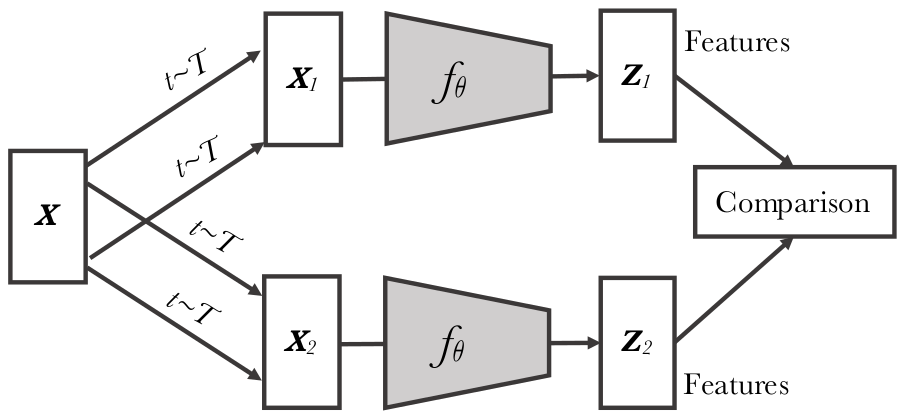
\includegraphics[width=0.4\textwidth]{./images/swav_contrastive.png}}
	\qquad
	\subcaptionbox{SWAV framework}
	{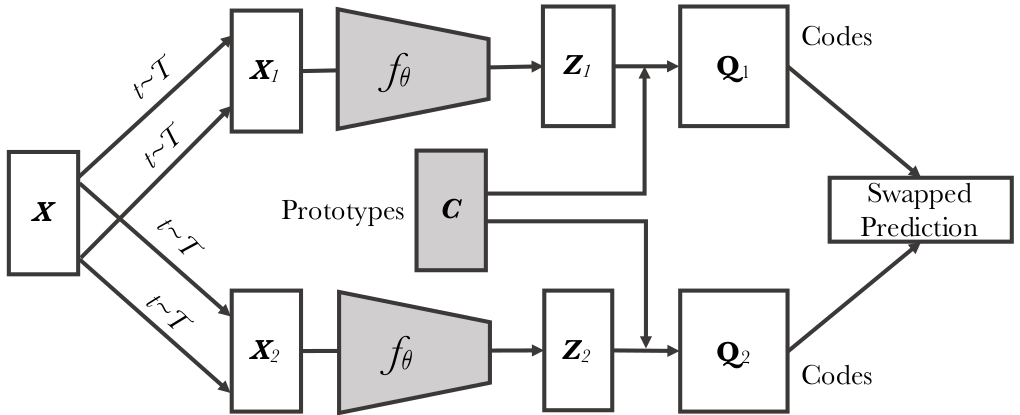
\includegraphics[width=0.4\textwidth]{./images/swav_prediction.png}}
	\caption{Difference between the classical contrastive learning framework with the one proposed in SWAV}

\end{figure}
The question now is how do we compute the codes? Given a batch of $B$ features $Z = [z_1, \dots, z_B]$ we want to map them to the prototypes $C= [C_1, \dots, C_K]$, obtaining the codes $Q = [q_1, \dots, q_B]$, where $Q$ is an $K\times B$ matrix where $Q_{i,j}$ can be viewed as the probability of feature $z_j$ to belong to the prototype $c_i$. We want to optimize $Q$ to maximize the similarity between features and prototypes, and this can be expressed in the following maximization problem:
\[ \max_{Q \in \mathcal{Q}} \Big\{ \Tr(Q^TC^TZ) + \epsilon H (Q) \Big\}\]
where $H(Q) = -\sum_i \sum_j Q_{i,j}\log Q_{i,j}$ and $\epsilon$ is a parameter that controls the smoothness of the mapping. The matrix $C^TZ$ contains the similarity of each feature vector and each prototype, since $(C^TZ)_{i,j} = c_i^Tz_j$.
%Hence we can r
%\[ \Tr(Q^TC^TZ) =  \sum_{i=1}^B\sum_{j=1}^K q_{j,i}(c^T_jz_i) = \sum_{i=1}^B\sum_{j=1}^K q_{j,i}\Big(\sum_{t=1}^Dc_{j,t}z_{i,t}\Big) \]
While solving the problem we need to avoid the trivial solution in which all the features are mapped to the same code. This can be achieved by imposing an equipartition constraint, which is basically saying that the number of feature vectors which are mapped to a given prototype has to be more or less the same for all the prototypes. In order to enforce the equal partitioning constraint the set $\mathcal{Q}$ is defined as:
\[ \mathcal{Q} = \{Q \in \mathbb{R}^{K \times B} | Q1_B = \frac{1}{k}1_k, Q^T1_K = \frac{1}{B}1_B \} \]
where $1_K$ denotes the $K$-dimensional vector where all the elements are 1. The solution to the optimization problem can be computed as:
\[ Q^* = \text{Diag}(u)\text{exp}\Big(\frac{C^TZ}{\epsilon}\Big)\text{Diag}(v) \]
where $u$ and $v$ are re-normalization vectors in $\mathbb{R}^K$ and $\mathbb{R}^B$, which can be computed with the Sinkhorn-Knopp algorithm.
